\documentclass[journal]{IEEEtran}
%% INFOCOM 2012 addition: 
\makeatletter
\def\ps@headings{%
\def\@oddhead{\mbox{}\scriptsize\rightmark \hfil \thepage}%
\def\@evenhead{\scriptsize\thepage \hfil \leftmark\mbox{}}%
\def\@oddfoot{}%
\def\@evenfoot{}}
\makeatother
\pagestyle{headings}
\usepackage{tabularx}
\usepackage{multirow}
\usepackage{booktabs}
\usepackage[utf8x]{inputenc}
\usepackage{framed, color}
\usepackage{mathtools}
\usepackage[super]{nth}
\usepackage{url}
\usepackage{subfig}
\usepackage{hyphenat}
\usepackage{ifthen}
\usepackage{tikz}
\usepackage[square, numbers, sort&compress]{natbib}
\usetikzlibrary{positioning,calc}
\usepackage{epstopdf}
\usepackage{nameref}
\usepackage{chngcntr}
\usepackage{amsmath}
\usepackage{graphicx}
\usepackage{caption}
\usepackage{adjustbox}
\usepackage{soul}
\usepackage{authblk}

\usepackage{algorithm}
\usepackage[noend]{algpseudocode}

\def\remove#1{}
\newcommand\ed[1]{{\color{red}#1}}

%\setremarkmarkup{\textcolor{red}{\bf{[#2]}}}


\counterwithin*{paragraph}{subsubsection} % removes paragraph from the subsubsections
\counterwithin*{paragraph}{section}
%\captionsetup[figure]{labelfont=bf,textfont={bf}}
%\captionsetup[table]{font=bf,position=below}


\begin{document}

 
\title{Measuring the Real Capacity of Lightning Channels}
 \author[1]{Marcelo Bagnulo} 
 \author[1]{Alberto  Garc\'{i}a-Mart\'{i}nez}
 \author[1]{Stefano Angieri}
 \author[2]{Antonio Fern\'{a}ndez Anta}
 \affil[1]{Universidad Carlos III de Madrid}
 \affil[2]{IMDEA Networks Institute}
 \renewcommand\Authands{ and }
 
 \maketitle


%\input{abstract}


\section{Introduction}
\input{Introduction}

\section{Off-line payment channels}
This section describes the mechanisms implemented in the Lightning network to support payments.

We model the Lightning network as a undirected graph $\langle N,C \rangle$, being N the Lightning \textit{nodes} and $C$ the \textit{channels}, that allow payments between two nodes.
Although the funding supporting a lightning channel is provisioned by one of the two nodes it connects,
it allows transactions started by any of them provided that the node initiating the transaction has enough positive balance. 
Therefore, Lightning channels are deemed to be \textit{bidirectional}.
We denote the channels as $C_{i,j}$, to represent a channel between $N_i$ and $N_j$, 
starting for convenience with the node that provisioned the funds (i.e., $N_{i}$ for $C_{i,j}$). 
As many channels can be set between the same pair of nodes, we denote them as $C'_{i,j}$, $C''_{i,j}$, etc.
Figure~\ref{fig:lightning-topology} shows an example of a Lightning topology.
% There can be more than 1 channel between two nodes
We define the capacity of channel $C_{i,j}$ from $N_i$ to $N_j$, denoted $\lambda_{i,j}$, 
%($\lambda'_{i,j}$, etc.), 
the amount of currency that can be transferred from $N_i$ to $N_j$ at the current moment. 
Then, with $\Lambda_{i,j}$ we denote the initial amount of currency funded by node $N_i$,
\begin{equation}
    \lambda_{j,i} = \Lambda_{i,j} - \lambda_{i,j}
\end{equation}

\begin{figure}[h!]
    \centering
    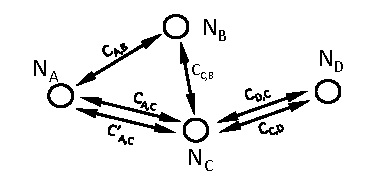
\includegraphics[width=0.95\linewidth]{img/lightning-topology.pdf}
    \caption{Example of Lightning topology}
    \label{fig:lightning-topology}
\end{figure}

The Lightning network~\cite{poon2016bitcoin} allows payments between nodes $N_i$ and $N_k$ that are not directly connected through a channel,
by means of relying in a sequence of nodes that act as intermediary parties.
The first node in the path must transfer the desired amount (plus appropriate fees) to the second, this to the third, and so on, until the destination receives the payment. 
Consensus on the completion of this operation is achieved by a sequence of pair-wise agreements, 
called bilateral \textit{hash time locked contracts}~\cite{BOLT_5_transaction_handling},
that guarantee that either every node involved receives the corresponding amount, or no one does.
These agreements are carried off-chain, in the sense that do not need to be registered in the blockchain to be trusted, 
although they can be when a channel is closed. 
%The mechanism ensures that either all the nodes receive the prove of the transaction, or neither of them can claim that …


To issue a transaction, the sender defines the intermediate channels through which the transaction will proceed. 
This path must be complete, in the sense that every channel traversed must be specified in advance.
Such a forwarding mechanism is usually known as \textit{strict source routing}~\cite{BOLT_4_onion_routing}.
To be able to discover channels, and thus build paths, nodes connect to other nodes already part of the network and exchange routing information. 
When a node connects first to a node part of the Lightning network, it receives the list of nodes and channels known by its peer~\cite{BOLT_7_routing_gossip}. 
Channel information includes source and destination channel endpoints (e.g., $i$ and $j$, respectively) 
and policy information referred to the channels: the funding capacity $\Lambda_{i,j}$ for the channel, the fee required for performing a payment, or the time lock during which the transaction [???]. 
The advertised capacity value for a channel $C_{i,j}$ corresponds to the value $\Lambda_{i,j}$ committed in the funding transaction creating the channel. 
Besides this initial information, nodes receive and propagate updates such as new channels added or channels closed.

When two nodes $N_i$ and $N_j$ have established a Lightning connection, they can negotiate the set up a new channel. 
In this negotiation, they build a multisignature Bitcoin address, so that the associated funds can only be retrieved under the agreement of both parties~\cite{poon2016bitcoin}.
Then, one of the nodes, e.g., $N_i$, performs a transaction in the Bitcoin blockchain, the funding transaction, to the multisignature address. 
The value of this transaction is the maximum amount of currency that can be transferred from $N_i$ to $N_j$.
The channel can now be advertised to other nodes, with the capacity set in the funding transaction, and the fees that they will apply to payments over the channel, that they exchanged in the channel setup negotiation.

Once created the channel, $N_i$ (and later $N_j$, when it has positive balance) can start issuing payments. 
These payments are executed as contracts they sign to each other, which are tied to time conditions (time-locks), in a way that any of the parties can eventually write the contract as a blockchain transaction that is executed to distribute the funds according to the last agreement and close the channel~\cite{BOLT_5_transaction_handling}. 
However, the channel does not need to be closed after a single transaction, but the contracts exchanged off-line (without blockchain registry) can keep an updated view of the balance of the parties over time.

Nodes willing to initiate a payment to a destination not directly connected through 
a channel use the routing information they have to compute 
paths with enough declared capacity to complete the transaction. 
Note that the current capacity can be different than this, as previous transactions may have altered the balance, 
and these changes are not advertised through the routing system.
Once defined the path by the initiator, a payment request 
is forwarded through it. 
When a node in the path receives the request, it checks if the next node is active - e.g., the node may be temporarily offline.
Then, the node checks if
actual channel capacity for the egressing channel suffices for the payment. 
If any of the checks fail, it reports an error to the source node, indicating the node that detected it, and the operation is aborted.
However, in case of low capacity, the node does not indicate the available capacity.

If all the nodes are connected, and have enough capacity, so the request arrives to the destination, then
the pair-wise hash time-locked contract machinery starts its operation~\cite{BOLT_2_channel_management, BOLT_5_transaction_handling}.




\section{Channel capacity measurement methodology}
\label{sec:methodology}
The exchange of channel information defined for the Lightning network includes information about the initial capacity of each channel. However, this capacity is not updated every time a transaction is performed.
We now present a methodology to be able to measure the actual capacity of a Lightning channel with low impact in the nodes and channels involved.
This methodology relies in performing transactions that traverse the channels to be measured, but which never complete, thus reverting the balance to the initial state. 

We use the information provided by the Lightning routing function to determine the nodes $N$ present at the lightning network, the channels $C$, and the declared channel capacities $\Lambda$.
Consider the topology depicted in Figure~\ref{fig:measurement-topology}.
We aim to measure the channel connecting $N_1$ and $N_2$. 
For this purpose, we deploy a new node to perform the measurement, node $N_0$, which will be the source of the measurement transaction.
For simplicity, we call the target channel $C_1$ (1 hop away from $N_0$), created with a funding transaction $\Lambda_1$, 
and with current capacity in the direction from $N_1$ to $N_2$ equal to $\lambda_1$ (which is the value to be measured).

$N_0$ attempts to establish a Lightning connection to node $N_1$. 
If node $N_1$ is reachable and accepts the connection (it may reject it due to the limitation in the number of connections or policy reasons), $N_0$ receives all the routing information $N_1$ has. 
Then $N_0$ starts the channel negotiation with node $N_1$. If successful, $N_0$ performs the funding transaction for the channel in the Bitcoin blockchain, with the multi signature derived from $N_0$ and $N_1$. 
This transaction must contain enough funds to test the capacity of the channel advertised by the routing system, $\Lambda_{1}$.



\begin{figure}[h!]
      \centering
      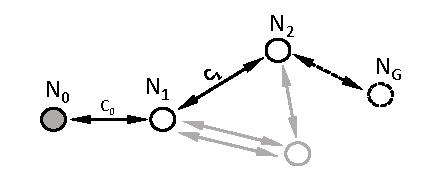
\includegraphics[width=0.99\linewidth]{img/measurement-topology.pdf}
      \caption{Measurement topology}
      \label{fig:measurement-topology}
\end{figure}

Once the funding transaction has completed (after the usual time to ensure Bitcoin consensus), 
$N_0$ starts measuring the capacity $\lambda_{1}$ by issuing a payment of $\lambda_t$, target capacity, 
to a \textit{ghost} node $N_G$.
This ghost node is a non-existent node, for which we generate a (non-existent) channel $C_{G}$ with a random identifier.
As the Lightning routing system is not aware of the ghost node, we request the routing system a route for $N_2$, 
and we modify the route to append the information corresponding to the last hop to $N_G$.
Thus, the resulting payment request, issued with a \texttt{sendtoroute} Lightning command, has a route $C_{0} \rightarrow C_1 \rightarrow C_{G}$. 
As neither $N_0$ nor $N_1$ validate the path with their routing information, the payment request is forwarded as long as enough capacity exits. 
However, when the request arrives to $N_2$, this node discards it, as it certainly knows there is no such node connected to it. 
Then the transaction is aborted, and an informative message is sent back to $N_0$.
Upon the reception of this message, we can deduce that $\lambda_t \leq \lambda_{0}$ and (more important to us) $\lambda_t \leq \lambda_{1}$, the channel to measure.
On the other hand, if $\lambda_t > \lambda_{1}$, then $N_1$ responds with a message indicating that there is not enough capacity in $C_1$, and also aborting the transference. 
In any of those cases, no hash-lock contracts are established, as they are only created from the payment receiver, in the direction to the issuer (would be created from $N_G$ to $N_2$, etc.), so no funds are blocked. 
Besides, as the computation requirements for this operation of checking and aborting are very low, the whole process is generally completed in less than a second. \ed{check!}

With the procedure described in the paragraph above we can test whether $\lambda_t \leq \lambda_{1}$. Let us call this procedure \textsc{EnoughCapacity}.
Then, we have that \textsc{EnoughCapacity}$(\lambda_t)=\mathit{True}$ if and only if $\lambda_t \leq \lambda_{1}$. 
We can use this procedure to devise the following strategy to obtain lower and upper bounds for the actual capacity of a channel $C_{1}$, as follows:
We start by assigning to $\lambda_t$ the initial target capacity advertised by the routing system, $\Lambda$, and we execute \textsc{EnoughCapacity}$(\lambda_t)$. If it returns $\mathit{True}$ (i.e., if the payment arrives to $N_2$), then we infer that the channel has the initial capacity.
%\footnote{We further check that there is no additional capacity to the advertised one by executing \textsc{EnoughCapacity} with $\lambda_t = \Lambda_{1} + \epsilon$, with $\epsilon$ a small value.} 
If it returns $\mathit{False}$ (the payment fails when arriving to $N_1$), then we move on checking another special case: whether the channel has no capacity left. To do so, we set $\lambda_t = \epsilon$ for a very small $\epsilon>0$ (since setting $\lambda_t = 0$ is not an option), and execute the procedure \textsc{EnoughCapacity}$(\lambda_t)$. If neither the capacity is the declared one, nor the channel is empty, 
we look for an intermediate capacity by an iterative binary search. 
The number of iterations of this loop is limited to $K$ (then, considering the test for the funding capacity and zero capacity, leads to a maximum number of payment requests per channel of $K+2$).
% For this, we perform an initial search to identify the order of magnitude of the current value, 
% by executing the procedure \texttt{EnoughCapacity} for $\Lambda_{1,2} / F^n$, with $F$ being a downscaling factor, 
% for $n: 1, 2, \ddots$, until a positive indication is reported.
% Then we execute a binary search that updates the maximum and minimum values observed so far. 
The result of the process is an estimation of the value for the actual capacity of the channel. 
We formalize the approach in Algorithm~\ref{alg:actual-capacity}.
% Note that the error can be expressed as $\frac{\lambda_{max} - \lambda_{min}}{2} = \Lambda 2^{-(K+1)}$}
The absolute error in the estimation made by the algorithm is $\epsilon$ for extreme values (either $\Lambda$ o 0 capacities), 
or $\Lambda \, 2^{-(K+1)}$ for the rest of the values, as resulting from a binary search. 
Therefore to obtain higher precision, higher values of $K$ can be used.

\begin{algorithm}
    \begin{algorithmic}[1]
    \Procedure{EstimateCapacity}{$C_{1}$, $K$}
    
    \State $\Lambda$ := \Call{GetFundingCapacity}{$C_{1}$}
    % \Comment{test initial capacity}
    \If{\Call{EnoughCapacity}{$\Lambda$}}
        % REMOVED CHECK FOR HIGHER CAPACITY: we observed some values for this
            % \If{not \Call{EnoughCapacity}{$\Lambda + \epsilon$}}  \Comment{Capacity is larger than advertised}
            %     \State return $\Lambda + \epsilon$
            % \Else
                \State return $\Lambda$
            % \EndIf
    \EndIf
    %\Comment{Test 0 capacity}
    \If{! \Call{EnoughCapacity}{$\epsilon$}}
        \State return 0
    \EndIf
    
    \State
    \State $\lambda_t$ := $\Lambda / 2$
    \State $\lambda_{max}$ := $\Lambda$
    \State $\lambda_{min}$ := 0
    \State counter :=0    
    \While {counter $< K$}
        \If{\Call{EnoughCapacity}{$\lambda_t$}}
        \State $\lambda_{min}$ := $\lambda_t$
        \State $\lambda_t$ := $\frac{\lambda_{min} + \lambda_{max}}{2}$
        \Else
            \State $\lambda_{max}$ := $\lambda_t$
            \State $\lambda_{t}$ := $\frac{\lambda_{min} + \lambda_{max}}{2}$
        \EndIf
        \State counter := counter + 1
    \EndWhile 
    

    \State return $\frac{\lambda_{min} + \lambda_{max}}{2}$
    \EndProcedure
    \end{algorithmic}
    \caption{Estimate $\lambda_{1}$ in a maximum of $K+2$ iterations with error $E = \Lambda \, 2^{-(K+1)}$ }
\label{alg:actual-capacity}
\end{algorithm}

Observe that, so far, we have not discussed the impact on the measurement of the node initially funding the channel (either $N_1$ or $N_2$).
% We have reasoned the capacity estimation procedure for the case $N_0$ connects to $N_1$ and measures
% a channel funded by $N_1$, i.e., measures $C_{1}$.
% It is straightforward to extend the procedure to the case, in which the channel was funded by $N_2$ (i.e., it is $C_{2,1}$). 
The fact is that, regardless of the node initially funding the channel, the transactions performed over the channel may result in any balance combination of the two directions, as far as the sum does not exceed \ed{[EQUALS??]} the value of the initial funding transaction. 
%This occurs regardless of the node performing the funding transaction.
% So, we set as maximum value of the capacity to be $\Lambda_{2,1}$, and we perform the tests. 
% To make the resulting capacity value independent of the node performing the funding transaction (either $N_1$ or $N_2$), we perform the following normalization for the measured value, $\lambda_{1,2}$: 
% If $N_1$, the node to which the measurement node attaches, was the node performing the funding transaction, we provide the measured capacity, $\lambda_{1,2}$.
% Conversely, if $N_2$ was the node which provisioned the funds, we provide $\lambda_{2,1}$, computed as $\Lambda_{2,1} - \lambda_{1,2}$. 
% In this way, regardless the node performing the funding transaction, the capacity estimation of the channel is positive, equal to the funding transaction value if no payment has been made, and 0 if the whole funded value has been transferred to the other node.

Finally, we comment the impact the experiment may have on the nodes under scrutiny.
The first cost is the computation resources required to establish a connection between $N_0$ and $N_1$. 
$N_1$ needs to send all the routing information to $N_0$. This process takes \ed{[Can we measure the mean time since we request a connection to when the connection is established? ]} 
Later, the nodes negotiate the setup of the channel. We deem this cost to be negligible compared to the exchange of routing information.
The second costs are associated to each capacity probe operation. For this case, 
note that the resources of the channel are not altered by the measure, as no transaction is finally performed. 
Besides, there is no temporal block of the resources, as the hash-lock contracts are not even established.
Additionally, we set a limit on the number of operations that can be requested to a node, to 3 operations per minute. 
The total number of transfers to perform with a node are limited to $K + 2$ times the number of channels of the node.

\section{Implementation and tests}
We have implemented the test suite over the \texttt{lnd} framework~\cite{lndDaemon}, 
a complete implementation of the Lightning node written in Go.
We use the command-line interface to access to routing information, 
gather routes and generate requests modified to suit to our measuring algorithm~\ref{sec:methodology}.

We have validated the testing methodology locally over the topology depicted in figure~\ref{fig:local-test-topology}, 
being each node an instance of the \texttt{lnd} daemon.
We create the channel to test, $C_{1,2}$, as follows: 
we command $N_1$ to execute a \texttt{connect} command in the Lightning command line interface 
(lncli) to $N_2$, and then we execute openchannel 
\ed{We dont know if openchannel negotiates or receives information from $N_2$ or not}
and it performs the funding transaction of the channel.

With this configuration, node $N_1$ advertises the funding capacity for the channel.
\ed{We are almost sure that $N_2$ does not advertise anything. Check what is the infomation $N_3$ receives}.

After this, $N_0$ can issue a transaction to $N_3$.
For this, it request a route. \ed{Check if this gathers information from $N_1$, and if so, which information. We think it does not receive information about the current balance, and we do not know which are the things it requests...but then we do not understand why it takes so much time and 
Execute strace for route request...}

If $N_3$ request a route for $N_0$, it does not receive any. However, we can build a route by generating manually information of the $N_2$ to $N_1$ hop, and then for the $N_1$ to $N_0$ hop.
If there is enough balance at $N_2$, then the transaction request is accepted and passed to $N_1$, and the same occurs from $N_1$ to $N_0$. Therefore, it is possible to perform the payment, but 
this way of paying is not provided out-of-the-box by the \texttt{lnd} suite.
\ed{we should know why is this}

We test with different capacities for the channel $C_{A,B}$, and execute the capacity estimation algorithm for path 
$\langle N_0$, $N_1$, $N_2$, $N_G \rangle$, and  path $\langle N_3$, $N_2$, $N_1$, $N_G \rangle$. 
We have checked in all cases that the sum of the measured capacities 
is consistent with the funding capacity (within the error margin of the capacity estimation).

We now test the case when one of the nodes is disconnected, i.e., $N_2$ for $\langle N_0$, $N_1$, $N_2$, $N_3 \rangle$ testing has been powered-off. 
...
Additionally, we show the result when $N_0$ is powered-off.

Test with $\epsilon$ (also for known balance, lower than funding capacity, test balance+$\epsilon$).

understand dust\_limit\_satoshis: 
Test dust\_limit\_satoshis 'is the threshold below which outputs should not be generated for this node's commitment or HTLC transactions (i.e., HTLCs below this amount plus HTLC transaction fees are not enforceable on-chain). This reflects the reality that tiny outputs are not considered standard transactions and will not propagate through the Bitcoin network.'
This may affect the fee, the amount to pay, or both.
So I would say $\epsilon=dust\dots$.
Which is the default value for this?



Other cases are: errors that may occur, how to generate them.
\ed{We don't know if there are behaviours specific to the daemon}

\begin{figure}[h!]
    \centering
    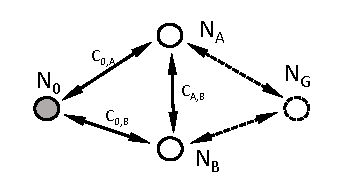
\includegraphics[width=0.99\linewidth]{img/local-test-topology.pdf}
    \caption{Local test topology}
    \label{fig:local-test-topology}
\end{figure}






\section{Experiment results}
\subsection{Things we do not understand from the results}
We connected to one mainnet node from the list of the top with most connections (lets name it Peer1), two nodes within the list of topmost value (peer2, peer3).
\begin{itemize}
\item Peer1 
    \begin{itemize}
    \item  has around 460 channels funded by it, most of them measured as 0 (the channels were spent)
    \item has around 30 funded by the remote nodes, most of them also empty (this means that the channels are almost full)
    \end{itemize}
    As a result, the amount of money spent is much higher than the amount of money received. Seems that this node is a \textbf{source of money}, not an intermediary point between others. Why?
    Similar results for peer2, peer3 (although not as unbalanced as this).
    \textit{To analyse this, follow the connections of peer1, and measure the channels this nodes have. Are spenders? are receivers? are transit?}
   
\end{itemize}



We discuss the results of the experiments performed in the Lightning \texttt{testnet} and 
the \texttt{mainnet}.

\subsection{testnet experiments}

We describe the experiments performed over the Lightning \texttt{testnet}, a Lightning network which operates with the 
testnet bitcoin tBTC, with a different blockchain to regular bitcoin.
We have connected to five nodes of the \texttt{testnet} network, and have measured the  capacity of the channels attached to them. 
Figure~\cite{fig:testnet_absolute_both_directions} 


\begin{figure}[h!]
    \centering
    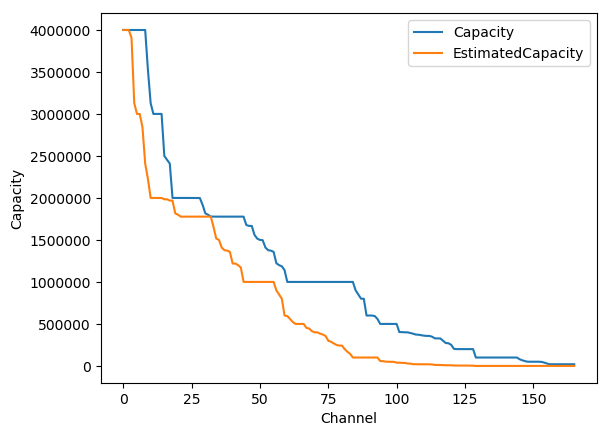
\includegraphics[width=0.99\linewidth]{img/testnet_absolute_both_directions.png}
    \caption{Testnet absolute capacities}
    \label{fig:testnet_absolute_both_directions}
\end{figure}


\subsection{mainnet experiments}
We now describe the tests performed in the full-value Lightning network, the \texttt{mainnet}, and the results obtained. 

Before starting the experiments, we first analyse the correspondence between the whole Lightning routing information 
(\texttt{mainnet}) and the channel status as recorded in the Bitcoin blockchain. 
In particular, we perform two checks: first, that every channel advertise in Lightning was funded in Lightning, but not closed; 
and second, if the capacity advertised by Lightning corresponds exactly with the amount of data annotated in the creation of the channel.
We observe that all the channels advertised are active (the channel was funded but not closed), 
and that the capacity advertised in Lightning for them corresponds to the funding transaction.

With the routing information for the Lightning network, we order the nodes in descending number of directly connected channels, 
and we follow the list until we establish a connection to 50 of them. 
In this phase, XXX nodes of this ordered list of top-most connected nodes rejected our attempt to connect. This could occur because of an excessive number of established connections.

For each of this nodes, we attempt to characterize all their channels, following the methodology presented in Section~\ref{sec:methodology}. 
The parameters we use for the estimation of the channel are $K=6$ (which gives an estimation error of less than 1\%) and $\epsilon = 10$ Satoshi.


In this way, we test XXX channels, the XXX\% of the total number of channels at the moment the experiment was performed. 
\ed{Some channels can appear twice, because they connect two tested nodes. Remove one for basic statistics, there is a specific paragraph about them below}

With the current state of the network, we can say that at least XXX1 Btcs have been exchanged through the channels measured (computed as $\sum{\Lambda}-\sum{\lambda}$). More value could have been exchanged in the channels, if payments go to the node performing the funding transaction. 
This is the YYY\% of the total provisioned value of the network. This lower bound for the amount of value transferred represents the XXX\% of the total value managed by the Lightning network ($\frac{\sum{\Lambda}-\sum{\lambda}}{\sum{\Lambda}}$). 
Figure 

The number of channels for which the measured capacity matches the funding capacity is XXX.
We have not observed any channel for which the measured capacity exceeds the funding capacity. % i.e., with positive value for $\Lambda + \epsilon $
The number of channels for which the whole amount of currency has been transferred from the node funding the channel to its peer, so that the balance is reversed from its original configuration, is XXX.

In Figure [FIG1] we depict the declared capacity for each of the channels tested and the measured capacity. In Figure [FIG2] we provide 

FIG1:
Bar graph with x-axis=channels, y=declared/measured capacity (declared > measured); ordered in x  axis by decreasing declared capacity.
Caption: Funding capacity and measured capacity for the tested channels.

FIG2:
SAME as FIG1, but with normalized funding capacity to 1.


There are XXX channels that connect two nodes tested in the experiment. These channels have been tested twice, in both directions. 
We match the values obtained in both directions, to asses that the values measured are consistent, i.e., within the margins stated by the errors of each one. 
% | measure1 - measure2| < 2 * single error

The total cost of the experiment was XXX Btc. This money was spent in the fees required to register in the blockchain the funding transaction to each of the measured nodes, and then the fee to  close the channel.
%The time required to perform the experiment was XXX.

\section{MeasureBIs}
Ideas to extend the measurement of lightning conference paper.

\ed{STEF: Test locally what happens if the node terminating the channel to meaure is not active).}

\ed{STEF: see what happens with max capacity + $\epsilon$}

\section{Lightning channel capacity measurement from a measuring node}
We describe a procedure to estimate node capacities of a path in the Lightning network. 
An estimation of the capacity is expressed as a lower bound/upper bound pair, namely $\langle \lambda_{min}, \lambda_{max} \rangle$ of the capacity this node have at a given instant. 
To do so, we connect a measurement node, $N_0$, under our control, to another Lightning nodes and perform different payment attempts to probe the network capacity.

Figure~\ref{fig:measurement-topology-extended} depicts the reference topology for this measurement: 
Lets consider a path formed by channels $C_0$ (between $N_0$ and $N_1$), $C_1$ (connecting $N_1$ and $N_2$), $C_2$, etc.
We assume that we know an estimation of the capacity of channels $C_0$, $C_1$, ..., $C_{i-1}$, and we want to estimate the capacity of $C_i$, i.e., $\lambda_i$.


\begin{figure}[h!]
    \centering
    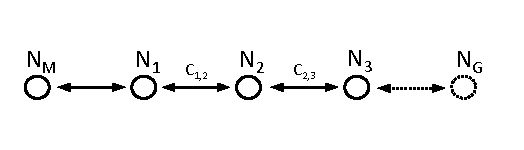
\includegraphics[width=0.95\linewidth]{img/measurement-topology-extended.pdf}
    \caption{Measurement topology extended to nodes two hops away}
    \label{fig:measurement-topology-extended}
\end{figure}


% We present EnoughCapacity
The measuring node can determine if the capacity of a channel $C_{x}$ exceeds a test value $t$ ($t<\lambda_i, \forall i < x$). 
To do so, $N_0$ performs a payment of $t$, to a \textit{ghost} node $N_G$.
This ghost node is a non-existent node, for which we generate a (non-existent) channel $C_{G}$ with a random identifier.
As the Lightning routing system is not aware of the ghost node, we 
 append to the path information provided by the routing system the information corresponding to the last hop to $N_G$.
Thus, the resulting payment request, issued with a \texttt{sendtoroute} Lightning command, has a route $C_{0} \rightarrow C_1 \rightarrow \ddots C_x, C_{G}$. 
As neither of the nodes from $N_0$ to $N_{i-1}$ validate the path with their routing information, the payment request is forwarded as long as enough capacity exits. 
However, if the request arrives to $N_i$, this node discards it, as it certainly knows there is no such channel connected to it. 
Then the transaction is aborted, and an informative a message is sent back to $N_0$.
Upon the reception of this message, we can deduce that $t \leq \lambda_{0}$, ... $t \leq \lambda_{i-1}$ and (more important to us) $t \leq \lambda_{i}$, the channel to measure.
On the other hand, if $t > \lambda_{i}$, then $N_i-1$ responds with a message indicating that there is no enough capacity, and also aborts the transference. 
In any of those cases, no hash-lock contracts are established, as they are only created from the payment receiver, in the direction to the issuer (would be created from $N_G$ to $N_i$, etc.), so no funds are blocked. 
Besides, as the computation requirements for this operation of checking and aborting are very low, the whole process is generally completed in less than a second.
We formalize the mechanism described above as a \textsc{EnoughCapacity} procedure, that takes a path, a channel to test, and a value, and returns whether the capacity at the channel is equal or higher than the test amount, or lower. 
The procedure reports an error if any of the precedent channels indicate that there is not enough capacity to make the payment progress.

We know present an algorithm to estimate $\langle \lambda_{i,min}, \lambda_{i,max} \rangle$ the capacity of channel $C_i$ in a path, assuming an estimation of the capacities of the previous channels in the path are known. 
In particular, we use the estimated capacity of the previous node, $\langle \lambda_{i,min}, \lambda_{i,max} \rangle$.
We also use $\Lambda_{i}$, the funding capacity of $C_{i}$, 
\ed{[Do this] which we obtain from matching the information of the Lightning routing system with the transactions performed into the blockchain. We have observed in some cases that the available capacity of a channel exceeds the capacity advertised by the Lightning routing system. This occurs because some nodes are configured to advertise a capacity value lower than the actual capacity commited to in the blockchain ledger.}

Apart from the lower/upper bounds for $\lambda_i$, the algorithm also indicates 
if the maximum value of the capacity is below or equal any tested capacity. 
This indicates when the capacities of the previous nodes prevented testing the maximum capacity.
We will exclude this nodes for statistics in which we count the channels having maximum capacity.

It does not aims to characterize capacities of channels that are behind others with empty (in the testing direction) capacity.


\begin{algorithm}
    \begin{algorithmic}[1]
    \Procedure{EstimateCapacity}{$\lambda_{i-1,min}$, $\lambda_{i-1,max}$, $\Lambda_{i}$, $K$}

    % Test 0 capacity, common for all cases
    % Note previous paths may have 0 capacity, or unknown (previous paths had 0 capacity)
    \If{$\lambda_{i-1, max} == 0$}
        \State return Error
        \Comment{Cannot estimate capacity if previous channel is empty}
    \EndIf

    % Test 0 capacity
    \If{! \Call{EnoughCapacity}{$C_{i}$, $\epsilon$}}
        % min, max, maximum could be tested
        \State return 0, 0, True
    \EndIf
        
    
    % We are not sure if the capacity of i is higher or equal than declared for i-1, just check
    \If{$\lambda_{i, max} \geq \Lambda_{i-1}$}
        % EnoughCapacity now has a target channel (i.e., the route stops there)

        \If {\Call{EnoughCapacity{$C_{i-1}$, $\Lambda_i$}}}
            \State $\lambda_{i-1, min}$ := $\Lambda_i$
        \EndIf
    \EndIf

    % We now know if the capacity of previous paths is  higher or not than funded for this
    \If{$\lambda_{x-1, min}  \geq \Lambda_x$ }
        % we can measure maximum values for x
        \If{\Call{EnoughCapacity}{$C_{i}$, $\Lambda_x$}}
            \If{not \Call{EnoughCapacity}{$C_{i}$, $\Lambda_i + \epsilon$}}  \Comment{Capacity is larger than advertised}
            % Maximum was tested, but result is not satisfactory
            \State return $\Lambda_i$, $\Lambda_i + \epsilon$, False
            \Else
                \State return $\Lambda_i$, $\Lambda_i$, True
            \EndIf
        \Else
            $\lambda_{i, max}$ := $\Lambda_i$
        \EndIf
    \Else
        % if i has maximum capacity, we cannot find it
        % Test if capacity is the maximum of the previous path
        \If{\Call{EnoughCapacity}{$C_{i}$, $\lambda_{i-1, min}$}}
            % This margin can be broad
            \State return $\lambda_{i-1, min}$, $\Lambda_i$, False
        \Else
            $\lambda_{i, max}$ := $\lambda_{i-1, min}$
        \EndIf
    \EndIf

    % Binary search, with proper adjusted maximum
    \State
    % lambda target for x
    \State $\lambda_{i,t}$ := $\lambda_{i, max} / 2$
    \State $\lambda_{i, min}$ := 0
    \State counter :=0    
    \While {counter $< K$}
        \If{\Call{EnoughCapacity}{$\lambda_{i,t}$}}
        \State $\lambda_{i,min}$ := $\lambda_{i,t}$
        \State $\lambda_{i,t}$ := $\frac{\lambda_{i, min} + \lambda_{i,max}}{2}$
        \Else
            \State $\lambda_{i,max}$ := $\lambda_t$
            \State $\lambda_{i,t}$ := $\frac{\lambda_{i,min} + \lambda_{i,max}}{2}$
        \EndIf
        \State counter := counter + 1
    \EndWhile 
    

    \State return $\lambda_{i,min}$, $\lambda_{i,max}$, True

    \EndProcedure
    \end{algorithmic}
    \caption{Find a lower and upper bound for  $\lambda_{x}$ in a maximum of $K+2$ iterations}
\label{alg:actual-capacity-x-hops}
\end{algorithm}


To increase the chances of a larger number of channels measured, $N_0$ connects with a capacity equal to the maximum transferable value defined by the Lightning specification, XXX. 

The algorithm presents the following properties: $\lambda_{i,min}$ is monotonically decreasing with $i$. 
However, $\lambda_{i,max}$ may increase, as it depends on the funding capacity of the channel.
We assume the error to be 0 when we match with the maximum capacity or empty channel. 
The error for a binary search is $min(\lambda_{i-1, min}, \Lambda_{i}) 2^{-(k+1)}$.
The error for the estimation of a channel $C_i$ with higher capacity than $\lambda_{i-1, min}$ is unbounded.
[Note that measures with T have a bounded error (either 0 or binary search error), while entries with F have unbounded error. When having to measures for the same channel, always prefer T over F.]

To illustrate the behavior of the algorithm, we consider the following case (for simplicity, we use small integer values for the funding and actual capacities):

\begin{table*}[]
    \begin{tabular}{llllllll}
     & $C_0$ & $C_1$ & $C_2$ & $C_3$ & $C_4$ & $C_5$ & $C_6$\\
    Maximum capacity for $C_i$, $\Lambda_i$ & 20 & 20 & 10 & 15 & 10 & 15 & 15 \\
    Current capacity for $C_i$, $\lambda_i$ & 20 & 18 & 10 & 5 & 10 & 10 & 3 \\
    $\lambda_{i, min}$ & - & 17.5 & 10 & 5 & 5 & 5 & 2.5 \\
    $\lambda_{i, max}$ & - & 20 & 10 & 6.5 & 10 & 15 & 3.125  \\
    Ensure maximum value is withing range & - & T & T & T  & F & F & T
    \end{tabular}
\end{table*}

To illustrate the behavior of the algorithm, we now execute the procedure with the channel configuration depicted in the table, and $K=3$. 
The maximum payment that can be made is 20, so this is the value for $\Lambda_0$ and $\lambda_0$.
We start with $C_1$. The test for empty capacity fails. Then, as the previous capacity is the maximum,
we can test $C_1$ for its funded capacity $\Lambda_1$, 20, which also fails.
Thus, a binary search is started within 0 and 20. Values of 10, 15, and 17.5 are tested, to generate a final bound pair of $<17.5, 20>$.

We now consider $C_2$. As $\lambda_{1,min}$, 17, is higher than $\Lambda_2$, 10, the mechanism tests the channel for its maximum capacity, which it succeeds. Therefore, the capacity estimation is $\langle 10,10 \rangle$.

For $C_3$, after testing the empty path, and being aware that the maximum capacity is 15, larger than the measured capacity for the precedent channel we start checking a value of 10. As the test indicates that the current capacity is lower, a binary search is conducted, to result in a value of $\langle 5, 6.25\rangle$. Note that even the value of 5 was specifically tested, the binary search cannot determine exact values, so a range (including the real value as a minimum) is reported.

We next process channel $C_4$. As the capacity of this channel is higher than the capacity of the previous, the algorithm responds with an estimation of $\langle 5, 10\rangle$.
For channel $C_5$, the situation is similar, with an estimation of $\langle 5, 15\rangle$

Finally, for $C_6$, when we test the minimum value of the previous channel, 5, it indicates that $\lambda_6$ is lower, so the binary search is started for the interval $\langle 0,5\rangle$, resulting in an estimation of $\langle 2.5, 3.125\rangle$.

\section{Evaluating Lightning network capacity}
Devise strategy for the measurements (to which nodes I should connect).

For measuring the channel capacity in the Lightning network, we propose the following strategy: 
We select the node with more channels of the highest funding capacity attached, according to the routing information.    
Then, we perform the process described in the previous section for channel estimation. 
We annotate the information in the routing graph. Then, we select the top node with a highest number of channels of the highest funding capacity for which no capacity estimation has been performed.
We estimate the channel capacities, annotate, and repeat the procedure until every channel has been characterized.

We first perform a 'dry run' of this scheme over the routing information data. For this case, we consider that the current capacity is equivalent to the funding capacity, although the nodes performing the measurement do not know this in advance. 
In figure [FIG] we show the number of channels characterized by this mechanism. 

[FIG] 
Draw the ccdf of the number of 
- total number of channels characterized
- number of  channels characterized as T
- number of channels characterized as F
x-axis: each round, from first to last.

We observe that... (maybe with few nodes it is enough to characterize most of the channels)
Decide with this how many rounds we may need in the real case.

We now apply the same scheme to real measures over the lightning network. 
We now observe ...

[Same figure as previous for the number of channels characterized]

At the end of the characterization process, we observe (similar to the results of the other paper...)

In addition to the results of the other paper, add these results
- number of channels that we can characterize, \% of the total number. Count high quality values (=T). Should be quite high.
- insist in matching values for the same channel observed in different measurements. Prefer T values over F. Be careful, as values may change over time, and measurements from different points (=made at different time) may measure different values.
I think that matching values support our methodology, while non-matching can be everything (this is a win-win :-))

\section{Evaluating the evolution of Lightning channels capacity over time}
[When repeating a measure (measuring a channel for which we have a previous value), we can start by checking if the previous capacity holds, with a previous +/- $\epsilon$ test.]

% We cannot select many, as it takes some time to measure.
We select randomly 1,000 channels and we observe the evolution over time of their capacities. 

Measure Lightning channel capacity one day, the day after, next week, next month, and compare the variation in the channel balance. 
This is a lower bound on the amount of money moved by Lightning (may be there are changes that we are not observing, moving in one direction, in other, etc.) 
Can be used to estimate the maturity of the network.

For this measure, we want to measure many channels in a short period of time: it the measure takes long, we may not be fast enough to measure the channels from one day to the other. Besides, a snapshot of the state is more valuable if the information of all the channels correspond to the same time. 

To be efficient in the previous task, measuring many channels in short periods of time, 
we want to connect to the lowest number possible of nodes, as establishing a channel with them takes long time 
(bitcoin transaction to create the channel, then bitcoin transaction to remove it). 
We cannot have multiple channels in parallel, as each channel requires the temporal assignment of a large amount of money. 
Besides, each time a channel is established and removed, we spent money. 

Therefore, we could formulate the problem as develop an algorithm that measures all the network by connecting to the lowest possible number of existing nodes.



\section{Related Work}
Interledger as a system that tries to solve a problem similar to the one solved by lighting but potentially across coins \cite{Interledger}.

The basics of Lightning and the Lightning Network can be found in the Lightning Network In-Progress Specifications \cite{ln-spec}. In particular, the
Onion Routing Protocol used in the current version is described in \cite{BOLT_4_onion_routing}.
%
A description of how payments are routed and how to choose fees to obtain low user fees and good network performance is presented in \cite{dirouting}.

A study \cite{LightningStrikes} shows that the probability of success of routing a payment deceases sharply as the amount increases. 
%Este mismo articulo ha sido analizado en estos: 
%https://medium.com/novamining/analysis-of-the-lightning-network-routing-problems-reported-by-diar-6d7ac0410471
%https://bitcoinnews.com/100-success-rate-on-bitcoins-lightning-network-only-for-3-cents-or-less/
%https://cointelegraph.com/news/study-low-reliability-for-successfully-routing-payments-on-lightning-network
%Pero el metodo utilizado para sacar estos resultados ha sido contestado para los del DevTeam de lightning mismo: 
%https://thenextweb.com/hardfork/2018/06/26/lighting-network-transactions/
%Y esta es la respuesta:
%https://diar.co/response-to-lighting-labs-lightning-network-dev-teams/
The lighting developers expect to correct this issue with the usage of Atomic Multi-Path Payments (AMP) \cite{LightningStrikes,TNW}, which allows a large payment divided into multiple smaller parallel payments. AMP will only make the routing problem more important.


-------- Editing here

Referencias para el problema de routing: 
https://www.yours.org/content/the-lightning-network-routing-problem--explained-31e1ba7b38f5
https://www.trustnodes.com/2019/03/13/lightning-network-has-many-routing-problems-says-lead-dev-at-lightning-labs



Y esta es una serie de aritculos  que describen una esperiencia de testeo de lightning hecha por Andreas Brekken (CEO de shitcoin.com). 
Andreas ha montados nodos,  ha incrementado la capacidad de la red del 68% poniendo dinero en sus nodos y ha intentado de hacer varios pagos.  

https://medium.com/andreas-tries-blockchain/bitcoin-lightning-network-1-can-i-compile-and-run-a-node-cd3138c68c15
https://medium.com/andreas-tries-blockchain/bitcoin-lightning-network-2-we-must-first-become-the-lightning-network-49c46953c1d7

En la parte 3 de esta serie, insegna los problemas tenido en hacer pagos debidos al routing y a los bucles del los wallet.

https://medium.com/andreas-tries-blockchain/bitcoin-lightning-network-3-paying-for-goods-and-services-5d9c492b0eb2
https://medium.com/andreas-tries-blockchain/bitcoin-lightning-network-4-what-happens-when-you-close-half-of-the-lightning-network-b25b330dfad2

\section{Conclusions}
The Lightning network is still in its infancy in terms of usage. 
We have presented a simple methodology to measure the current capacity of a Lightning channel. 

For future work, we consider improving the methodology to measure channels that are not directly connected to the nodes the measurement node attaches to. In this way we could increase the number of channels that could be characterized, without increasing the cost of the experiment (resulting from the transactions in the blockchain required to establish and removing the measurement channel) and the time to perform the experiment (a large component is the time required to ensure consensus on the blockchain transaction used to open and close the channel). 

Besides increasing the number of measured channels, we are also interested in capturing the evolution of the capacities overtime. 
As we have noted, capacity measurement does not provide enough information to evaluate the amount of value that circulates over the network, as it only shows the current balance, but not the steps followed to reach to that balance.
By taking different snapshots over varying periods of time we aim to gather more information about the (now elusive) flow of currency across Lightning.

\small

\bibliographystyle{IEEEtran}
\bibliography{./references} 

\end{document}
